\documentclass[a4paper, openany]{memoir}

\usepackage[utf8]{inputenc}
\usepackage[T1]{fontenc} 
\usepackage[english]{babel}

\usepackage{fancyhdr}
\usepackage{float}

\usepackage{amsmath}
\usepackage{amsthm}
\usepackage{amssymb}
\usepackage{enumitem}
\usepackage{multicol}
\usepackage[bookmarksopen=true,bookmarksopenlevel=2]{hyperref}
\usepackage{tikz}
\usepackage{listings}
\usepackage{xcolor}
\usepackage{indentfirst}
% \usepackage{graphicx}

\pagestyle{fancy}
\fancyhf{}
\fancyhead[LE]{\leftmark}
\fancyhead[RO]{\rightmark}
\fancyhead[RE, LO]{Algorithmics I}
\fancyfoot[LE, RO]{\thepage}
\fancyfoot[RE, LO]{Pete Gautam}

\definecolor{codegreen}{rgb}{0,0.6,0}
\definecolor{codegray}{rgb}{0.5,0.5,0.5}
\definecolor{codepurple}{rgb}{0.58,0,0.82}
\definecolor{backcolour}{rgb}{0.95,0.95,0.92}

\lstdefinestyle{thestyle}{
    backgroundcolor=\color{backcolour},
    basicstyle=\ttfamily\footnotesize,
    keywordstyle=\color{red!80}\bfseries,
    ndkeywordstyle=\color{blue!80}\bfseries,
    identifierstyle=\color{black},
    commentstyle=\color{codegreen},
    stringstyle=\color{codepurple},
    breakatwhitespace=false,
    breaklines=true,
    captionpos=b,
    keepspaces=true,
    numberstyle=\tiny\color{codegray},
    numbers=left,
    numbersep=2pt,
    showspaces=false,
    showstringspaces=false,
    showtabs=false,          
    tabsize=2
}

\lstdefinelanguage{pseudocode}{ 
    keywords={new, return, this, null, if, in, while, else, for, get, set, class, and, or, not, range},
    ndkeywords={int, bool, char, List, String, Node, Queue, Set, Tree, Map, Code, void, true, false},
    sensitive=true,
    comment=[l]{//},
    morecomment=[s]{/*}{*/},
    morestring=[b]',
    morestring=[b]"
}

\lstset{style=thestyle}

\usetikzlibrary{shapes, positioning}

\chapterstyle{thatcher}

\setcounter{chapter}{1}

\begin{document}

\chapter{String and Text Algorithms}
\section{Text Compression}
Text compression is a special case of data compression. It aims to save disk space and transmission time. Text compression, unlike image, audio or video, must be lossless, i.e. the original file must be recoverable without error. So, for a compression algorithm, there has to be a decompression algorithm to transform the compression file back into the original file unchanged.

There are two main approaches to text compression- statistical and dictionary. The compression ratio is the value $x/y$, where $x$ is the size of the compressed file and $y$ is the size of the original file. For example, if we compress a 10MB file into a 2MB file, the compression ratio is $2/10 = 0.2$. The percentage of space saved is $(1 - 0.2) \cdot 100\% = 80\%$. Usually, the space saved is between $40\%$ and $60\%$.

\subsection{Huffman Encoding}
This is a classical statistical method of text compression. In this approach, a fixed (ASCII) code is replaced by a variable length code. Every character is represented by a unique codeword (a bit string). This approach compresses the file because we represent frequently occurring characters with shorter codewords.

The code has the prefix property. That is, no codeword is a prefix of another. This allows us to decompress the text unambiguously- it is clear when to stop reading a bit string and how to interpret it.

This approach is based on the Huffman tree, which is a proper binary tree. Each character is represented by a leaf node. The codeword for a character is given by the path from the root to the appropriate leaf (left=0 and right=1). The prefix property follows from this. Following the bit string is equivalent to traversing the binary tree. Since all the characters are leaf nodes, there is no path that can correspond to more than one character. Moreover, we know we have reached the end when we encounter a leaf node.

We will now illustrate how to create the Huffman tree. So, assume that we have the following character frequency table for some text.
\begin{table}[H]
    \centering
    \begin{tabular}{|ccccccccccccc|}
        \hline
        \texttt{Space} & \texttt{E} & \texttt{A} & \texttt{T} & \texttt{I} & \texttt{S} & \texttt{R} & \texttt{O} & \texttt{N} & \texttt{U} & \texttt{H} & \texttt{C} & \texttt{D} \\
        15 & 11 & 9 & 8 & 7 & 7 & 7 & 6 & 4 & 3 & 2 & 1 & 1 \\
        \hline
    \end{tabular}
    \caption{A character frequency table.}
\end{table}
\noindent We shall construct a Huffman tree for these characters based on their frequency. We start by placing the characters (along with their frequency) in the tree, as leaf nodes.
\begin{figure}[H]
    \centering
    \begin{tikzpicture}[
        level 1/.style = {sibling distance = 4cm, level distance=0cm},
        level 2/.style = {sibling distance = 3cm, level distance=0cm},
        level 3/.style = {sibling distance = 2cm, level distance=1.2cm},
        level 4/.style = {sibling distance = 1cm, level distance=1.2cm},
    ]
    \node {}
    child {
        node[] {}
        child {
            node[] {}
            child {
                node[] {}
                child {
                    node[draw, label={-90:I}] {7}
                    edge from parent[draw=none]
                }
                child {
                    node[draw, label={-90:\texttt{S}}] {7}
                    edge from parent[draw=none]
                }
                edge from parent[draw=none]
            }
            child {
                node[] {}
                child {
                    node[] {}
                    child {
                        node[] {}
                        child {
                            node[] {}
                            child {
                                node[draw, label={-90:\texttt{C}}] {1}
                                edge from parent[draw=none]
                            }
                            child {
                                node[draw, label={-90:\texttt{D}}] {1}
                                edge from parent[draw=none]
                            }
                            edge from parent[draw=none]
                        }
                        child {
                            node[draw, label={-90:\texttt{H}}] {2}
                            edge from parent[draw=none]
                        }
                        edge from parent[draw=none]
                    }
                    child {
                        node[draw, label={-90:\texttt{U}}] {3}
                        edge from parent[draw=none]
                    }
                    edge from parent[draw=none]
                }
                child {
                    node[draw, label={-90:\texttt{R}}] {7}
                    edge from parent[draw=none]
                }
                edge from parent[draw=none]
            }
            edge from parent[draw=none]
        }
        child {
            node[] {}
            child {
                node[draw, label={-90:\texttt{E}}] {11}
                edge from parent[draw=none]
            }
            child {
                node[] {}
                child {
                    node[draw, label={-90:\texttt{O}}] {6}
                    edge from parent[draw=none]
                }
                child {
                    node[draw, label={-90:\texttt{N}}] {4}
                    edge from parent[draw=none]
                }
                edge from parent[draw=none]
            }
            edge from parent[draw=none]
        }
        edge from parent[draw=none]
    }
    child {
        node[] {}
        child {
            node[draw, label={-90:\texttt{Space}}] {15}
            edge from parent[draw=none]
        }
        child {
            node[] {}
            child {
                node[draw, label={-90:\texttt{T}}] {8}
                edge from parent[draw=none]
            }
            child {
                node[draw, label={-90:\texttt{A}}] {9}
                edge from parent[draw=none]
            }
            edge from parent[draw=none]
        }
        edge from parent[draw=none]
    };
    \end{tikzpicture}
    \caption{A Huffman tree to be formed for the character frequency tree above.}
\end{figure}
\noindent Next, we add a new parent to nodes of the smallest weights. The weight of this parent is equal to the sum of the weights of the child nodes.
\begin{figure}[H]
    \centering
    \begin{tikzpicture}[
        level 1/.style = {sibling distance = 4cm, level distance=0cm},
        level 2/.style = {sibling distance = 3cm, level distance=0cm},
        level 3/.style = {sibling distance = 2cm, level distance=1.2cm},
        level 4/.style = {sibling distance = 1cm, level distance=1.2cm},
    ]
    \node {}
    child {
        node[] {}
        child {
            node[] {}
            child {
                node[] {}
                child {
                    node[draw, label={-90:I}] {7}
                    edge from parent[draw=none]
                }
                child {
                    node[draw, label={-90:\texttt{S}}] {7}
                    edge from parent[draw=none]
                }
                edge from parent[draw=none]
            }
            child {
                node[] {}
                child {
                    node[] {}
                    child {
                        node[] {}
                        child {
                            node[circle, draw] {2}
                            child {
                                node[draw, label={-90:\texttt{C}}] {1}
                            }
                            child {
                                node[draw, label={-90:\texttt{D}}] {1}
                            }
                            edge from parent[draw=none]
                        }
                        child {
                            node[draw, label={-90:\texttt{H}}] {2}
                            edge from parent[draw=none]
                        }
                        edge from parent[draw=none]
                    }
                    child {
                        node[draw, label={-90:\texttt{U}}] {3}
                        edge from parent[draw=none]
                    }
                    edge from parent[draw=none]
                }
                child {
                    node[draw, label={-90:\texttt{R}}] {7}
                    edge from parent[draw=none]
                }
                edge from parent[draw=none]
            }
            edge from parent[draw=none]
        }
        child {
            node[] {}
            child {
                node[draw, label={-90:\texttt{E}}] {11}
                edge from parent[draw=none]
            }
            child {
                node[] {}
                child {
                    node[draw, label={-90:\texttt{O}}] {6}
                    edge from parent[draw=none]
                }
                child {
                    node[draw, label={-90:\texttt{N}}] {4}
                    edge from parent[draw=none]
                }
                edge from parent[draw=none]
            }
            edge from parent[draw=none]
        }
        edge from parent[draw=none]
    }
    child {
        node[] {}
        child {
            node[draw, label={-90:\texttt{Space}}] {15}
            edge from parent[draw=none]
        }
        child {
            node[] {}
            child {
                node[draw, label={-90:\texttt{T}}] {8}
                edge from parent[draw=none]
            }
            child {
                node[draw, label={-90:\texttt{A}}] {9}
                edge from parent[draw=none]
            }
            edge from parent[draw=none]
        }
        edge from parent[draw=none]
    };
    \end{tikzpicture}
\end{figure}
\noindent In this case, we connect \texttt{C} and \texttt{D} with a parent node of weight 2. Now, we connect the new node with H to get a node of weight 4.
\begin{figure}[H]
    \centering
    \begin{tikzpicture}[
        level 1/.style = {sibling distance = 4cm, level distance=0cm},
        level 2/.style = {sibling distance = 3cm, level distance=0cm},
        level 3/.style = {sibling distance = 2cm, level distance=1.2cm},
        level 4/.style = {sibling distance = 1cm, level distance=1.2cm},
    ]
    \node {}
    child {
        node[] {}
        child {
            node[] {}
            child {
                node[] {}
                child {
                    node[draw, label={-90:I}] {7}
                    edge from parent[draw=none]
                }
                child {
                    node[draw, label={-90:\texttt{S}}] {7}
                    edge from parent[draw=none]
                }
                edge from parent[draw=none]
            }
            child {
                node[] {}
                child {
                    node[] {}
                    child {
                        node[circle, draw] {4}
                        child {
                            node[circle, draw] {2}
                            child {
                                node[draw, label={-90:\texttt{C}}] {1}
                            }
                            child {
                                node[draw, label={-90:\texttt{D}}] {1}
                            }
                        }
                        child {
                            node[draw, label={-90:\texttt{H}}] {2}
                        }
                        edge from parent[draw=none]
                    }
                    child {
                        node[draw, label={-90:\texttt{U}}] {3}
                        edge from parent[draw=none]
                    }
                    edge from parent[draw=none]
                }
                child {
                    node[draw, label={-90:\texttt{R}}] {7}
                    edge from parent[draw=none]
                }
                edge from parent[draw=none]
            }
            edge from parent[draw=none]
        }
        child {
            node[] {}
            child {
                node[draw, label={-90:\texttt{E}}] {11}
                edge from parent[draw=none]
            }
            child {
                node[] {}
                child {
                    node[draw, label={-90:\texttt{O}}] {6}
                    edge from parent[draw=none]
                }
                child {
                    node[draw, label={-90:\texttt{N}}] {4}
                    edge from parent[draw=none]
                }
                edge from parent[draw=none]
            }
            edge from parent[draw=none]
        }
        edge from parent[draw=none]
    }
    child {
        node[] {}
        child {
            node[draw, label={-90:\texttt{Space}}] {15}
            edge from parent[draw=none]
        }
        child {
            node[] {}
            child {
                node[draw, label={-90:\texttt{T}}] {8}
                edge from parent[draw=none]
            }
            child {
                node[draw, label={-90:\texttt{A}}] {9}
                edge from parent[draw=none]
            }
            edge from parent[draw=none]
        }
        edge from parent[draw=none]
    };
    \end{tikzpicture}
\end{figure}
\noindent Now, we can either connect the parent node of weight 4 with \texttt{U}, or we can connect \texttt{N} with \texttt{U}. It does not matter which one we choose- we will just end up with a different compression algorithm in that case.
\begin{figure}[H]
    \centering
    \begin{tikzpicture}[
        level 1/.style = {sibling distance = 4cm, level distance=0cm},
        level 2/.style = {sibling distance = 3cm, level distance=0cm},
        level 3/.style = {sibling distance = 2cm, level distance=1.2cm},
        level 4/.style = {sibling distance = 1cm, level distance=1.2cm},
    ]
    \node {}
    child {
        node[] {}
        child {
            node[] {}
            child {
                node[] {}
                child {
                    node[draw, label={-90:I}] {7}
                    edge from parent[draw=none]
                }
                child {
                    node[draw, label={-90:\texttt{S}}] {7}
                    edge from parent[draw=none]
                }
                edge from parent[draw=none]
            }
            child {
                node[] {}
                child {
                    node[circle, draw] {7}
                    child {
                        node[circle, draw] {4}
                        child {
                            node[circle, draw] {2}
                            child {
                                node[draw, label={-90:\texttt{C}}] {1}
                            }
                            child {
                                node[draw, label={-90:\texttt{D}}] {1}
                            }
                        }
                        child {
                            node[draw, label={-90:\texttt{H}}] {2}
                        }
                    }
                    child {
                        node[draw, label={-90:\texttt{U}}] {3}
                    }
                    edge from parent[draw=none]
                }
                child {
                    node[draw, label={-90:\texttt{R}}] {7}
                    edge from parent[draw=none]
                }
                edge from parent[draw=none]
            }
            edge from parent[draw=none]
        }
        child {
            node[] {}
            child {
                node[draw, label={-90:\texttt{E}}] {11}
                edge from parent[draw=none]
            }
            child {
                node[] {}
                child {
                    node[draw, label={-90:\texttt{O}}] {6}
                    edge from parent[draw=none]
                }
                child {
                    node[draw, label={-90:\texttt{N}}] {4}
                    edge from parent[draw=none]
                }
                edge from parent[draw=none]
            }
            edge from parent[draw=none]
        }
        edge from parent[draw=none]
    }
    child {
        node[] {}
        child {
            node[draw, label={-90:\texttt{Space}}] {15}
            edge from parent[draw=none]
        }
        child {
            node[] {}
            child {
                node[draw, label={-90:\texttt{T}}] {8}
                edge from parent[draw=none]
            }
            child {
                node[draw, label={-90:\texttt{A}}] {9}
                edge from parent[draw=none]
            }
            edge from parent[draw=none]
        }
        edge from parent[draw=none]
    };
    \end{tikzpicture}
\end{figure}
\noindent In this case, we will connect \texttt{U} to the parent node. 
\noindent We can continue on connecting nodes until we end up with no parentless nodes.
\begin{figure}[H]
    \centering
    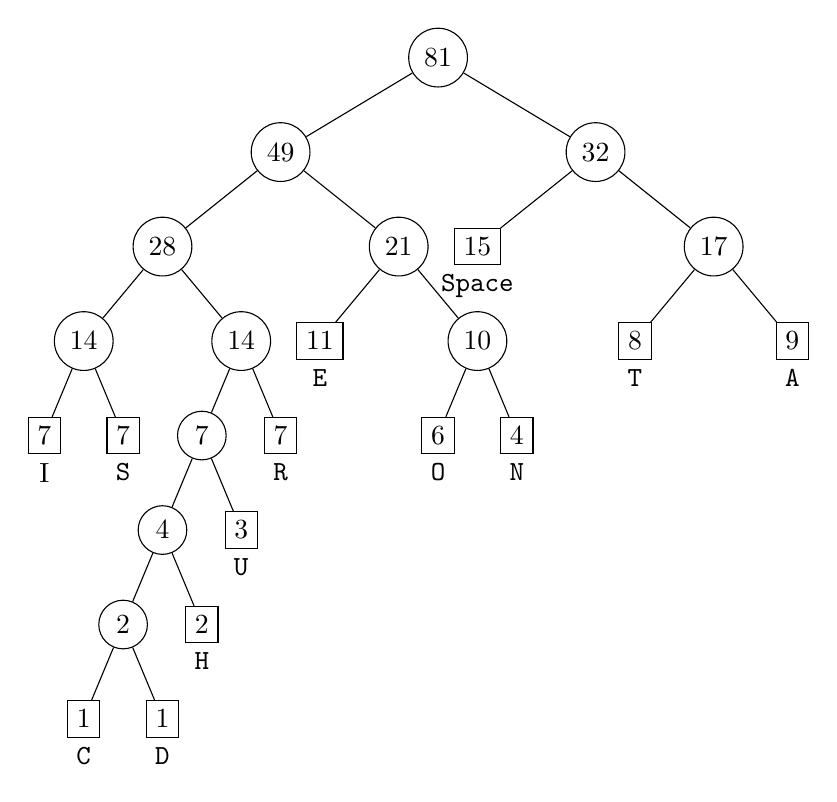
\begin{tikzpicture}[
        level 1/.style = {sibling distance = 4cm},
        level 2/.style = {sibling distance = 3cm},
        level 3/.style = {sibling distance = 2cm},
        level 4/.style = {sibling distance = 1cm},
        level distance=1.2cm,
    ]
    \node[circle, draw] {81}
    child {
        node[circle, draw] {49}
        child {
            node[circle, draw] {28}
            child {
                node[circle, draw] {14}
                child {
                    node[draw, label={-90:I}] {7}
                }
                child {
                    node[draw, label={-90:\texttt{S}}] {7}
                }
            }
            child {
                node[circle, draw] {14}
                child {
                    node[circle, draw] {7}
                    child {
                        node[circle, draw] {4}
                        child {
                            node[circle, draw] {2}
                            child {
                                node[draw, label={-90:\texttt{C}}] {1}
                            }
                            child {
                                node[draw, label={-90:\texttt{D}}] {1}
                            }
                        }
                        child {
                            node[draw, label={-90:\texttt{H}}] {2}
                        }
                    }
                    child {
                        node[draw, label={-90:\texttt{U}}] {3}
                    }
                }
                child {
                    node[draw, label={-90:\texttt{R}}] {7}
                }
            }
        }
        child {
            node[circle, draw] {21}
            child {
                node[draw, label={-90:\texttt{E}}] {11}
            }
            child {
                node[circle, draw] {10}
                child {
                    node[draw, label={-90:\texttt{O}}] {6}
                }
                child {
                    node[draw, label={-90:\texttt{N}}] {4}
                }
            }
        }
    }
    child {
        node[circle, draw] {32}
        child {
            node[draw, label={-90:\texttt{Space}}] {15}
        }
        child {
            node[circle, draw] {17}
            child {
                node[draw, label={-90:\texttt{T}}] {8}
            }
            child {
                node[draw, label={-90:\texttt{A}}] {9}
            }
        }
    };
    \end{tikzpicture}
    \caption{The Huffman tree for the character frequency given above.}
\end{figure}
Using the tree, we can construct Huffman code for each character. Going to the left corresponds to a \texttt{0} while going to the right corresponds to a \texttt{1}. This gives us the following table.
\begin{table}[H]
    \centering
    \begin{tabular}{|ccccccc|}
        \hline
        \texttt{Space} & \texttt{E} & \texttt{A} & \texttt{T} & \texttt{I} & \texttt{S} & \texttt{R} \\
        \texttt{10} & \texttt{010} & \texttt{111} & \texttt{110} & \texttt{0000} & \texttt{0001} & \texttt{0011} \\
        \hline
        & \texttt{O} & \texttt{N} & \texttt{U} & \texttt{H} & \texttt{C} & \texttt{D} \\
        & \texttt{0110} & \texttt{0111} & \texttt{00101} & \texttt{001001} & \texttt{0010000} & \texttt{0010001} \\
        \hline
    \end{tabular}
    \caption{The Huffman code for each character.}
\end{table}
\noindent Clearly, the more frequently occurring values have a shorter code. Also, no code is a prefix of another. For example, if we read \texttt{111010}, it can only correspond to \texttt{AE}.

The pseudocode for constructing the Huffman tree is given below.
\lstinputlisting[language=pseudocode]{src/huffmanTree.psc}

Huffman encoding is an optimal algorithm. To see this, we consider the weighted path length (WPL) of a tree $T$. This is the sum of the weight multiplied by the distance from the root product. For example, in the tree above, the WPL is
\[7 \times 4 + 7 \times 4 + 1 \times 7 + 1 \times 7 + 2 \times 6 + \cdots + 9 \times 3 = 279.\]
Huffman tree has minimum WPL over all binary trees with the given leaf weights. For a given set of frequencies, there need not be a unique Huffman tree, but all Huffman trees have the same WPL. 

The weighted path length is the number of bits in the compressed file. This is because every character has a length (corresponding to the length of the edges) along with a frequency. So, the total number of bits is equal to the sum of this product for every node, i.e. the weighted path length. The Huffman tree has the minimum WPL, so this algorithm minimises the size of the compressed file as much as possible.

Now, we analyse the algorithm. Assume that we have a text of length $n$ containing $m$ distinct characters. It takes $O(n)$ time to find the frequency. It takes $O(m \log m)$ time to construct the code, for example, using a (min) heap to store the parentless nodes and their weights. Initially, we need to build the heap- this takes $O(m)$ time. An iteration takes $O(\log m)$ time- we find and remove the two minimum weights, and insert a new weight. There are $m-1$ iterations before the heap is left with one element. Overall, the algorithm is $O(n + m \log m)$. The number of characters $m$ is essentially a constant, so it is really $O(n)$. 

We also need to consider compression and decompression. Compression uses a code table (an array of codes indexed by a character). It takes $O(m \log m)$ to build the table as we have $m$ characters with paths of length $\leq \log m$ since it is a binary tree. It takes $O(n)$ to compress- there are $n$ characters in the text, so we lookup the code $n$ times. Overall, it takes $O(n \log m) + O(n)$ time. Decompression uses the tree directly, so it is $O(n \log m)$ as we traverse $n$ times a path of length $\leq \log m$.

In order to decompress, we must keep some representation of the Huffman tree along with the compressed file. An alternative to storing the tree is using a fixed set of frequencies based on typical values for text. But, this will usually reduce the compression ratio. We can also use adaptive Huffman coding. Here, the (same) tree is built and adapted by the compressor and the decompressor as characters get encoded and decoded. This slows the compression and the decompression, but not by much if done in a clever way.

\subsection{LZW Encoding}
LZW is a dictionary-based method. The dictionary is a collection of strings, each with a codeword that represents it. The codeword is a bit pattern, but it can be interpreted as a non-negative integer as well. Whenever a codeword is outputted during compression, what is written to the compression file is the bit pattern. It is a number of bits determined by the current codeword length. So, at any point, all bit patterns are the same length.

The dictionary is built dynamically during compression (and decompression). Initially, the dictionary contains all possible strings of length 1. During the algorithm, the dictionary is closed under prefixes. So, if the string $s$ is represented in the dictionary, so is every prefix of $s$. Therefore, a trie is an ideal representation of the dictionary. Every node in the trie represents a `word' in the dictionary. This makes trie an effective data structure to use during the algorithm.

At any given point during compression (or decompression), there is a current codeword length $k$. So, there are exactly $2^k$ distinct codewords available. This limits the size of the dictionary. However, the codeword length can be incremented as necessay, thereby doubling the number of available codewords. The initial value of $k$ should be large enough to encode all strings of length 1.

The pseudocode for LZW compression is given below.
\lstinputlisting[language=pseudocode]{src/lzwCompression.psc}
Also, the pseudocode for LZW decompression is given below.
\lstinputlisting[language=pseudocode]{src/lzwDecompression.psc}

Since tries are trees, when we find the longest string present starting at $s[i]$, we just need to go down a branch instead of searching a new string from the start. This means that the tries implementation is very efficient.

There are many variants to LZW compression. We can have a constant codeword length, where the dictionary has fixed capacity. When it is full, we stop adding more codewords. The one we saw above is the dynamic version, where we start with the shortest reasonable codeword length. When the dictionary becomes full, we add 1 to the current codeword length- it doubles the number of codewords. It does not affect the sequence of codewords already present. We may specify a maximum codeword length, as increasing the size indefinitely may become counter-productive. Another variant is the LRU version, where the current string replaces the least recently used string in the dictionary when the dictionary is full and the codeword length is maximal.

We will illustrate the algorithm on the following text: \texttt{GACGATACGATACG}. Assuming 2 bits per each character, the file size is 28 bits. There are 4 different characters present, so the initial codeword length $k = 2$. The initial dictionary is \texttt{A:00}, \texttt{C:01}, \texttt{G:10} and \texttt{T:11}.

We start from the beginning of the text. \texttt{G} is the longest string we can find in the dictionary starting there. We keep track of the codeword for \texttt{G}- 10. We add to the dictionary the longest string and the next character, i.e. \texttt{GA}. It gets code 100. We have now increased the codeword length from 2 to 3.

We are now at position 2. The longest string here is \texttt{A}- its codeword is 000. We add to dictionary \texttt{AC}- its codeword is 101. We can continue this process until we reach the final position. This process is summarised in the table below.
\begin{table}[H]
    \centering
    \begin{tabular}{|c|c|c|c|c|}
        \hline
        position & longest string & b & add to dictionary & code \\
        \hline
        1 & \texttt{G} & 10 & \texttt{GA} & 100 \\
        \hline
        2 & \texttt{A} & 000 & \texttt{AC} & 101 \\
        \hline
        3 & \texttt{C} & 001 & \texttt{CG} & 110 \\
        \hline
        4 & \texttt{GA} & 100 & \texttt{GAT} & 111 \\
        \hline
        6 & \texttt{T} & 011 & \texttt{TA} & 1000 \\
        \hline
        7 & \texttt{AC} & 0101 & \texttt{ACG} & 1001 \\
        \hline
        9 & \texttt{GAT} & 0111 & \texttt{GATA} & 1010 \\
        \hline
        12 & \texttt{ACG} & 1001 & - & - \\
        \hline
    \end{tabular}
    \caption{The LZW compression table for the text \texttt{GACGATACGATACG}}
\end{table}
\noindent The compressed file is the concatenation of the codewords $b$. So, it is 100000011 00011010101111001. This has file size of 26 bits.

The decompression algorithm also builds the same dictionary as the compression algorithm, but it is one step out of phase. The implementation of the LZW decompression algorithm is given below.

We will illustrate the decompression algorithm by decompressing the bit string above. We start with the same dictionary at the start and the same codeword length. So, the codeword length is 2 and the dictionary is \texttt{A:0}, \texttt{C:1}, \texttt{G:2} and \texttt{T:3}. Note that the bit strings are in decimal here- they do not need to be.

First, we search for a code. The codeword length is 2, so we have the bit 10. This corresponds to \texttt{G}. At this point, we do not add anything to the dictionary. We keep track of the old string. 

The dictionary is full, so we increment the size- the codeword length is now 3. We then look at the next 3 bits- we find 000. This corresponds to the character \texttt{A}. So, we keep track of \texttt{A}. We also add to the dictionary the old string and the first character of the new string- \texttt{GA}. It gets the code 4.

We can continue this process and decode the string. The following table summarises the process.
\begin{table}[H]
    \centering
    \begin{tabular}{|c|c|c|c|c|c|c|}
        \hline
        position & old string & dictionary code & string & add to dictionary & code \\
        \hline
        1 & \texttt{-} & 10 & \texttt{G} & \texttt{-} & - \\
        \hline
        3 & \texttt{G} & 000 & \texttt{A} & \texttt{GA} & 100 \\
        \hline
        6 & \texttt{A} & 001 & \texttt{C} & \texttt{AC} & 101 \\
        \hline
        9 & \texttt{C} & 100 & \texttt{GA} & \texttt{CG} & 110 \\
        \hline
        12 & \texttt{GA} & 011 & \texttt{T} & \texttt{GAT} & 111 \\
        \hline
        15 & \texttt{T} & 0101 & \texttt{AC} & \texttt{TA} & 1000 \\
        \hline
        19 & \texttt{AC} & 0111 & \texttt{GAT} & \texttt{ACG} & 1001 \\
        \hline
        23 & \texttt{GAT} & 1001 & \texttt{ACG} & \texttt{GATA} & 1010 \\
        \hline
    \end{tabular}
    \caption{The LZW decompression table for the encoded text 10000001100011010101111001.}
\end{table}
\noindent Concatenating the string, we get back the original text: \texttt{GACGATACGATACG}.

During decompression, it is possible to encounter a codeword that is not (yet) in the dictionary. This is possible because decompression is `out of phase' with compression. But, in that case, it is possible to deduce what the string it must represent- it is the old string at this point and the first character of the new string.

The complexity of both compression and decompression is $O(n)$, where $n$ is the length of the text. The algorithm essentially involves just one pass through the text. We do not need to search for longest strings in the dictionary.
\newpage

\section{String Distance}
Before discussing string distance, we will consider some string notations. If a string $s$ is of length $m$, then $s[i]$ is the $i+1$-th element of the string if $0 \leq i < m$. Also, for $-m \leq i < 0$, $s[i]$ refers to $m-i$-th element of the string. The slice $s[i:j]$ refers to the substring from $s[i]$ (included) to $s[j]$ (excluded). If either value is missing, then we start from the start or we finish in the end respectively.

The $j$-th prefix of a string is the first $j$ characters, i.e. $s[:j]$. The $0$-th prefix $s[:0]$ is the empty string $\epsilon$. Also, the $j$-th suffix is the last $j$ characters, i.e. $s[-j:]$. Like in the case of prefixes, the $0$-th suffix $s[0:]$ is the empty string.

We can look at two strings $s$ and $t$ and consider the distance between them. This is the smallest number of basic operations that we need to perform in order to transform $s$ into $t$. There are 3 basic operations- insertion of a character (e.g. \texttt{red} $\to$ \texttt{re{\color{red} a}d}), deletion of a character (e.g. \texttt{{\color{red} h}eat} $\to$ \texttt{eat}) and substitution of a character (e.g. \texttt{{\color{red} d}ead} $\to$ \texttt{{\color{red} b}ead}).

For example, consider the strings $s = \texttt{abadcdb}$ and $t = \texttt{acbacacb}$. The following is an alignment between $s$ and $t$.
\begin{table}[H]
    \centering
    \begin{tabular}{|c|ccccccccc|}
        \hline
        $s$ & \texttt{a} & \texttt{{\color{red}-}} &  \texttt{b} & \texttt{a} & \texttt{{\color{red} d}} & \texttt{c} & \texttt{{\color{red} d}} & \texttt{{\color{red} -}} & \texttt{b} \\
        $t$ & \texttt{a} & \texttt{{\color{red} c}} & \texttt{b} & \texttt{a} & \texttt{{\color{red} -}} & \texttt{c} & \texttt{{\color{red} a}} & \texttt{{\color{red} c}} & \texttt{b} \\
        \hline
    \end{tabular}
    \caption{The alignment of the two strings \texttt{abadcdb} and \texttt{acbacacb}. The mismatches are shown in red.}
\end{table}
\noindent An alignment illustrates how we can transform the string $s$ into $t$- we add a \texttt{c}; we remove a \texttt{d}; we substitute a \texttt{d} with an \texttt{a}; and we add a \texttt{c}. Therefore, the distance between $s$ and $t$ is less than or equal to 4. It turns out that it is not possible for the distance to be 3 or lower- we will prove this later.

The string distance algorithm uses dynamic programming. The problem is solved by building up solutions to subproblems of ever increasing size. This is often called the tabular method since we build a table of relevant values. Eventually, one of the values in the table gives the required answer.

In the dynamic programming algorithm, let $s$ and $t$ be the two strings whose distance we want to compute. Let $d(i, j)$ be the distance between the $i$-th prefix of $s$ and the $j$-th prefix of $t$. The distance between $s$ and $t$ is then $d(m, n)$, where $m$ is the length of $s$ and $n$ the length of $t$.

The recurrence relation defining the distance is given by the distance between the shorter prefixes- $d(i-1, j-1)$ (which accounts for equal characters or substitution), $d(i, j-1)$ (which accounts for deletion of a character from $t$) and $d(i-1, j)$ (which accounts for deletion of a character from $s$).

The base case here is that $d(i, 0) = i$ and $d(j, 0) = j$. This reflects the fact that the distance from the empty string to a string of length $k$ is $k$- we need to delete $k$ elements from the string. In an optimal alignment of the $i$-th prefix of $s$ with the $j$-th prefix of $t$, the last position of the alignment must either be a match or one of substitution, insertion and deletion. If there is a match, then we do not need to increment the distance. Otherwise, we increment the distance by 1. The recurrence relation is therefore given as
\[d(i, j) = \begin{cases}
d(i-1, j-1) & s[i-1] = t[j-1] \\
1 + \min(d(i-1, j-1), d(i, j-1), d(i-1, j)) & \text{otherwise}.
\end{cases}\]

The dynamic programming algorithm for string distance follows immediately from the formula. We fill in the entries of an $m \times n$ table either row by row or column by column. The algorithm has both time and space complexity $O(mn)$, as determined by the size of the table. We can easily reduce the space complexity to $O(m+n)$ by just keeping track of the previous column. To get the optimal alignment, we can use a traceback in the table. It is less obvious how this can be done using $O(m+n)$ space, but it turns out that this is still possible.

We illustrate this algorithm with an example. Assume we want to find the distance between string \texttt{acbacacb} and \texttt{abadcdb}. We initialise the table by the base case.
\begin{table}[H]
    \centering
    \begin{tabular}{|c|c|c|c|c|c|c|c|c|c|}
        \hline
         & $\epsilon$ & \texttt{a} & \texttt{c} & \texttt{b} & \texttt{a} & \texttt{c} & \texttt{a} & \texttt{c} & \texttt{b} \\
        \hline
        $\epsilon$ & 0 & 1 & 2 & 3 & 4 & 5 & 6 & 7 & 8 \\
        \hline
        \texttt{a} & 1 & & & & & & & & \\
        \hline
        \texttt{b} & 2 & & & & & & & & \\
        \hline
        \texttt{a} & 3 & & & & & & & & \\
        \hline
        \texttt{d} & 4 & & & & & & & & \\
        \hline
        \texttt{c} & 5 & & & & & & & & \\
        \hline
        \texttt{d} & 6 & & & & & & & & \\
        \hline
        \texttt{b} & 7 & & & & & & & & \\
        \hline
    \end{tabular}
\end{table}
\noindent For example, the entry $(0, 3)$ tells us that the distance between the empty string $\epsilon$ and the prefix \texttt{acb} is 3. We now fill the next row.
\begin{table}[H]
    \centering
    \begin{tabular}{|c|c|c|c|c|c|c|c|c|c|}
        \hline
        & $\epsilon$ & \texttt{a} & \texttt{c} & \texttt{b} & \texttt{a} & \texttt{c} & \texttt{a} & \texttt{c} & \texttt{b} \\
        \hline
        $\epsilon$ & 0 & 1 & 2 & 3 & 4 & 5 & 6 & 7 & 8 \\
        \hline
        \texttt{a} & 1 & {\color{brown} 0} & {\color{red} 1} & 2 & 3 & 4 & 5 & 6 & 7 \\
        \hline
        \texttt{b} & 2 & & & & & & & & \\
        \hline
        \texttt{a} & 3 & & & & & & & & \\
        \hline
        \texttt{d} & 4 & & & & & & & & \\
        \hline
        \texttt{c} & 5 & & & & & & & & \\
        \hline
        \texttt{d} & 6 & & & & & & & & \\
        \hline
        \texttt{b} & 7 & & & & & & & & \\
        \hline
    \end{tabular}
\end{table}
\noindent The entry $(1, 1)$ is a 0- since $s[0] = t[0]$, we take the entry at $(0, 0)$. On the other hand, the entry $(1, 2)$ is a 1- since $s[0] \neq t[1]$, we increment by 1 the smallest of $(1, 1)$, $(0, 1)$ and $(0, 2)$, which is $(1, 1)$. 
\pagebreak

\noindent We then move onto the next row.
\begin{table}[H]
    \centering
    \begin{tabular}{|c|c|c|c|c|c|c|c|c|c|}
        \hline
         & $\epsilon$ & \texttt{a} & \texttt{c} & \texttt{b} & \texttt{a} & \texttt{c} & \texttt{a} & \texttt{c} & \texttt{b} \\
        \hline
        $\epsilon$ & 0 & 1 & 2 & 3 & 4 & 5 & 6 & 7 & 8 \\
        \hline
        \texttt{a} & 1 & 0 & 1 & 2 & 3 & 4 & 5 & 6 & 7 \\
        \hline
        \texttt{b} & 2 & {\color{red} 1} & 1 & {\color{brown} 1} & 2 & 3 & 4 & 5 & 6 \\
        \hline
        \texttt{a} & 3 & & & & & & & & \\
        \hline
        \texttt{d} & 4 & & & & & & & & \\
        \hline
        \texttt{c} & 5 & & & & & & & & \\
        \hline
        \texttt{d} & 6 & & & & & & & & \\
        \hline
        \texttt{b} & 7 & & & & & & & & \\
        \hline
    \end{tabular}
\end{table}
\noindent Here, the entry $(2, 1)$ is a 1- since $s[1] \neq t[0]$, we add 1 to the lowest distance from the closest 3. Also, the entry $(2, 3)$ is a 1- since $s[1] = t[2]$, we just take the value in $(1, 2)$. We can continue this process and fill out the rest of the table.
\begin{table}[H]
    \centering
    \begin{tabular}{|c|c|c|c|c|c|c|c|c|c|}
        \hline
         & $\epsilon$ & \texttt{a} & \texttt{c} & \texttt{b} & \texttt{a} & \texttt{c} & \texttt{a} & \texttt{c} & \texttt{b} \\
        \hline
        $\epsilon$ & 0 & 1 & 2 & 3 & 4 & 5 & 6 & 7 & 8 \\
        \hline
        \texttt{a} & 1 & 0 & 1 & 2 & 3 & 4 & 5 & 6 & 7 \\
        \hline
        \texttt{b} & 2 & 1 & 1 & 1 & 2 & 3 & 4 & 5 & 6 \\
        \hline
        \texttt{a} & 3 & 2 & 2 & 2 & 1 & 2 & 3 & 4 & 5 \\
        \hline
        \texttt{d} & 4 & 3 & 3 & 3 & 2 & 2 & 3 & 4 & 5 \\
        \hline
        \texttt{c} & 5 & 4 & 3 & 4 & 3 & 2 & 3 & 3 & 4 \\
        \hline
        \texttt{d} & 6 & 5 & 4 & 4 & 4 & 3 & 3 & 4 & 4 \\
        \hline
        \texttt{b} & 7 & 6 & 5 & 4 & 5 & 4 & 4 & 4 & {\color{brown} 4} \\
        \hline
    \end{tabular}
\end{table}
\noindent The entry at the final row, final column is 4. So, the distance between the strings $s$ and $t$ is 4.

The pseudocode for this algorithm is given below.
\lstinputlisting[language=pseudocode]{src/stringDistance.psc}

To compute the optimal alignment between $s$ and $t$, we enter the traceback phase. This traces a path in the table from the bottom right to the top left. We take a path from one entry to a previous one based on what led to the value of this node, i.e. whether there was a match and we took the diagonal, or whether the minimum value was above, etc.

A vertical step in the table refers to a deletion from $s$; a horizontal step is an insertion in $s$; and diagonal steps are matches (if the distance does not change) or substitutions. The traceback is not necessarily unique since more than one of the entries could be the minimum value. This implies that there can be more than one optimal alignment.

From the table above, we get the following traceback table.
\begin{table}[H]
    \centering
    \begin{tabular}{|c|c|c|c|c|c|c|c|c|c|}
        \hline
         & $\epsilon$ & \texttt{a} & \texttt{c} & \texttt{b} & \texttt{a} & \texttt{c} & \texttt{a} & \texttt{c} & \texttt{b} \\
        \hline
        $\epsilon$ & {\color{red} 0} & 1 & 2 & 3 & 4 & 5 & 6 & 7 & 8 \\
        \hline
        \texttt{a} & 1 & {\color{red} 0} & {\color{red} 1} & 2 & 3 & 4 & 5 & 6 & 7 \\
        \hline
        \texttt{b} & 2 & 1 & 1 & {\color{red} 1} & 2 & 3 & 4 & 5 & 6 \\
        \hline
        \texttt{a} & 3 & 2 & 2 & 2 & {\color{red} 1} & 2 & 3 & 4 & 5 \\
        \hline
        \texttt{d} & 4 & 3 & 3 & 3 & 2 & {\color{red} 2} & {\color{red} 3} & 4 & 5 \\
        \hline
        \texttt{c} & 5 & 4 & 3 & 4 & 3 & 2 & 3 & {\color{red} 3} & 4 \\
        \hline
        \texttt{d} & 6 & 5 & 4 & 4 & 4 & 3 & 3 & {\color{red} 4} & 4 \\
        \hline
        \texttt{b} & 7 & 6 & 5 & 4 & 5 & 4 & 4 & 4 & {\color{red} 4} \\
        \hline
    \end{tabular}
\end{table}
\noindent This gives us the following alignment.
\begin{table}[H]
    \centering
    \begin{tabular}{|c|ccccccccc|}
        \hline
        & d & h & d & d & d & h & d & v & d \\
        \hline
        $s$ & \texttt{a} & \texttt{\color{red} -} & \texttt{b} & \texttt{a} & \texttt{\color{red} d} & \texttt{\color{red} -} & \texttt{c} & \texttt{\color{red} d} & \texttt{b} \\
        $t$ & \texttt{a} & \texttt{\color{red} c} & \texttt{b} & \texttt{a} & \texttt{\color{red} c} & \texttt{\color{red} a} &\texttt{c} & \texttt{\color{red} -} & \texttt{b} \\
        \hline
    \end{tabular}
    \caption{An optimal traceback of the dynamic programming algorithm. The value d refers to a diagonal step; h a horizontal step; and v a vertical step.}
\end{table}

Below is another example, where we compute the distance between the strings \texttt{saturday} and \texttt{sunday}.
\begin{table}[H]
    \centering
    \begin{tabular}{|c|c|c|c|c|c|c|c|}
        \hline
        & $\epsilon$ & \texttt{s} & \texttt{u} & \texttt{n} & \texttt{d} & \texttt{a} & \texttt{y} \\
        \hline
        $\epsilon$ & 0 & 1 & 2 & 3 & 4 & 5 & 6 \\
        \hline
        \texttt{s} & 1 & 0 & 1 & 2 & 3 & 4 & 5 \\
        \hline
        \texttt{a} & 2 & 1 & 1 & 2 & 3 & 3 & 4 \\
        \hline
        \texttt{t} & 3 & 2 & 2 & 2 & 3 & 4 & 4 \\
        \hline
        \texttt{u} & 4 & 3 & 2 & 3 & 3 & 4 & 5 \\
        \hline
        \texttt{r} & 5 & 4 & 3 & 3 & 4 & 4 & 5 \\
        \hline
        \texttt{d} & 6 & 5 & 4 & 4 & 3 & 4 & 5 \\
        \hline
        \texttt{a} & 7 & 6 & 5 & 5 & 4 & 3 & 4 \\
        \hline
        \texttt{y} & 8 & 7 & 6 & 6 & 5 & 4 & 3 \\
        \hline
    \end{tabular}
\end{table}
\noindent The distance is therefore 3. We can traceback to find the optimal path.
\begin{table}[H]
    \centering
    \begin{tabular}{|c|c|c|c|c|c|c|c|}
        \hline
        & $\epsilon$ & \texttt{s} & \texttt{u} & \texttt{n} & \texttt{d} & \texttt{a} & \texttt{y} \\
        \hline
        $\epsilon$ & {\color{red} 0} & 1 & 2 & 3 & 4 & 5 & 6 \\
        \hline
        \texttt{s} & 1 & {\color{red} 0} & 1 & 2 & 3 & 4 & 5 \\
        \hline
        \texttt{a} & 2 & {\color{red} 1} & 1 & 2 & 3 & 3 & 4 \\
        \hline
        \texttt{t} & 3 & {\color{red} 2} & 2 & 2 & 3 & 4 & 4 \\
        \hline
        \texttt{u} & 4 & 3 & {\color{red} 2} & 3 & 3 & 4 & 5 \\
        \hline
        \texttt{r} & 5 & 4 & 3 & {\color{red} 3} & 4 & 4 & 5 \\
        \hline
        \texttt{d} & 6 & 5 & 4 & 4 & {\color{red} 3} & 4 & 5 \\
        \hline
        \texttt{a} & 7 & 6 & 5 & 5 & 4 & {\color{red} 3} & 4 \\
        \hline
        \texttt{y} & 8 & 7 & 6 & 6 & 5 & 4 & {\color{red} 3} \\
        \hline
    \end{tabular}
\end{table}
\noindent So, the optimal alignment is provided below.
\begin{table}[H]
    \centering
    \begin{tabular}{|c|cccccccc|}
        \hline
        & d & v & v & d & d & d & d & d \\
        \hline
        $s$ & \texttt{s} & \texttt{{}\color{red} a} & \texttt{\color{red} t} & \texttt{u} & \texttt{\color{red} r} & \texttt{d} & \texttt{a} & \texttt{y} \\
        $t$ & \texttt{s} & \texttt{\color{red} -} & \texttt{\color{red} -} & \texttt{u} & \texttt{\color{red} n} & \texttt{d} &\texttt{a} &\texttt{y} \\
        \hline
    \end{tabular}
    \caption{Optimal alignment of the dynamic programming algorithm.}
\end{table}
\newpage

\section{String and pattern searching}
String and pattern searching is where we search a (long) text for a (short) string. We will focus on finding a substring within the string.

\subsection{Brute Force}
% Given a text $t$ (of length $n$) and a string $s$ (of length $m$), we are trying to find the position of the first occurrence (if any) of $s$ in $t$.
The naive brute force algorithm (also known as exhaustive search) sets the current starting position in the string to be zero. It then compares the string and substring characters left-to-right until the entire substring is matches, or we have a mismatch. If there is a complete match, then we return the right index. Otherwise, we advance the starting position by 1 and repeat. The pseudocode for this algorithm is given below.
\lstinputlisting[language=pseudocode]{src/bruteForce.psc}

We illustrate the algorithm with an example. In the figure below, we try to find \texttt{ababaca} in \texttt{bacbabababacaab}.
\begin{figure}[H]
    \centering
    \begin{tabular}{ccccccccccccccc}
        \texttt{b} & \texttt{a} & \texttt{c} & \texttt{b} & \texttt{a} & \texttt{b} & \texttt{a} & \texttt{b} & \texttt{a} & \texttt{b} & \texttt{a} &\texttt{c} & \texttt{a} & \texttt{a} & \texttt{b} \\
        \hline
        \texttt{{\color{red} a}} & \texttt{b} & \texttt{a} & \texttt{b} & \texttt{a} & \texttt{c} & \texttt{a} \\
        & \texttt{{\color{brown} a}} & \texttt{{\color{red} b}} & \texttt{a} & \texttt{b} & \texttt{a} & \texttt{c} & \texttt{a} \\
        & & \texttt{{\color{red} a}} & \texttt{b} & \texttt{a} & \texttt{b} & \texttt{a} & \texttt{c} & \texttt{a} \\
        & & & \texttt{{\color{red} a}} & \texttt{b} & \texttt{a} & \texttt{b} & \texttt{a} & \texttt{c} & \texttt{a} \\
        & & & & \texttt{{\color{brown} a}} & \texttt{{\color{brown} b}} & \texttt{{\color{brown} a}} & \texttt{{\color{brown} b}} & \texttt{{\color{brown} a}} & \texttt{{\color{red} c}} & \texttt{a} \\
        & & & & & \texttt{{\color{red} a}} & \texttt{b} & \texttt{a} & \texttt{b} & \texttt{a} & \texttt{c} & \texttt{a} \\
        & & & & & & \texttt{{\color{brown} a}} & \texttt{{\color{brown} b}} & \texttt{{\color{brown} a}} & \texttt{{\color{brown} b}} & \texttt{{\color{brown} a}} & \texttt{{\color{brown} c}} & \texttt{{\color{brown} a}}
    \end{tabular}
    \caption{Brute Force Search of the substring \texttt{ababaca} in the string \texttt{bacbabababacaab}. Red means a mismatch, while brown means a match.}
\end{figure}
We start checking from the beginning of the text. If there is a mismatch (i.e. the value we are checking in the string does not match the value in the text), then we restart, checking from the next value. We continue this until we find a match, or we have reached the end of the string.

We now analyse the algorithm. Assume that the string $t$ is of length $n$ and the substring $s$ is of length $m$. In the worst case, we reach the last character in the string before finding a mismatch, i.e. $s = \underbrace{\texttt{aa} \cdots \texttt{ab}}_{\text{length } m}$ and $t = \underbrace{\texttt{aa} \cdots \texttt{ab}}_{\text{length } n}$. We have $m$ character comparisons need at each $n - (m+1)$ positions in the text before we find the pattern. So, the complexity is $O(mn)$. In practice, the number of comparisons from each point will be small. For instance, it typically just takes 1 comparison to find a mismatch. So, we can expect $O(n)$ on average.

\subsection{KMP Algorithm}
Instead of using the brute force, we can use KMP algorithm for time complexity $O(m+n)$ in the worst case. It is an on-line algorithm, i.e. when we have compared a character in the string with a character in the substring, we never compare it to another character. 

To achieve this, we pre-process the string to build a border table. A border table is an array $b$ with entry $b[j]$ for each position $j$ of the string. If we have a mismatch at position $j$ in the string, we remain on the current character in the string. The border table tells us which character in the substring should next be compared with the current character in the string.

A substring of a string $s$ is a sequence of consecutive characters of $s$. If $s$ has length $n$, then $s[i:j]$ is a substring for valid $i$ and $j$. A prefix of $s$ is a substring that begins at position 0, i.e. $s[:j]$ for some $j$. A suffix of $s$ is a substring that ends at position $n-1$, i.e. $s[i:]$ for some $i$. 

A border of a string is a substring that is both a prefix and a suffix, but not the entire string. For example, if we have the string $s = \texttt{acacgatacac}$, then \texttt{ac} and \texttt{acac} are borders. In this case, the longest border is \texttt{acac}. Many strings do not have a border- their longest border is the empty string $\epsilon$.

The KMP algorithm requires the border table of the string pattern. In the border table $b$, the entry $b[j]$ contains the length of the longest border of $s[:j]$. For example, the border table for \texttt{ababaca} is given below.
\begin{table}[H]
    \centering
    \begin{tabular}{|c|c|c|c|c|c|c|}
        \hline
        \texttt{a} & \texttt{b} & \texttt{a} & \texttt{b} & \texttt{a} & \texttt{c} & \texttt{a} \\
        \hline
        0 & 0 & 0 & 1 & 2 & 3 & 0 \\
        \hline
    \end{tabular}
    \caption{The border table for the string \texttt{ababaca}.}
\end{table}
\noindent The first two values are 0 since the empty string and the character \texttt{a} have no border. Since the string \texttt{aba} has a border of size 1, the fourth entry is 1. Also, the longest border of \texttt{ababa} is \texttt{aba}. This is allowed even though the middle \texttt{a} is part of both the prefix and the suffix. So, the second last entry is 3.

We shall now illustrate how the KMP is better than the brute force. Assume that we are at a mistmatch, like in the case below.
\begin{figure}[H]
    \centering
    \begin{tabular}{cccccccccccccccccc}
        \texttt{a} & \texttt{g} & \texttt{a} & \texttt{g} & \texttt{{\color{gray} t}} & \texttt{c} & \texttt{a} & \texttt{t} & \texttt{a} & \texttt{a} & \texttt{c} & \texttt{g} & \texttt{a} \\
        \hline
         \texttt{{\color{brown} a}} & \texttt{{\color{brown} g}} & \texttt{{\color{brown} a}} &  \texttt{{\color{brown} g}} &  \texttt{{\color{red} g}}
    \end{tabular}
\end{figure}
\noindent In the brute-force case, we would advance the starting position by 1 and restart the search.
\begin{figure}[H]
    \centering
    \begin{tabular}{cccccccccccccccccc}
        \texttt{a} & \texttt{g} & \texttt{a} & \texttt{g} & \texttt{{\color{gray} t}} & \texttt{c} & \texttt{a} & \texttt{t} & \texttt{a} & \texttt{a} & \texttt{c} & \texttt{g} & \texttt{a} \\
        \hline
         \texttt{{\color{brown} a}} & \texttt{{\color{brown} g}} & \texttt{{\color{brown} a}} &  \texttt{{\color{brown} g}} &  \texttt{{\color{red} g}} \\
        & \texttt{a} & \texttt{g} & \texttt{a} & \texttt{g} & \texttt{g} 
    \end{tabular}
\end{figure}
\noindent In the brute force algorithm, we would have to compare the substring \texttt{gag} in the string again even though we have already matched those characters. However, the KMP algorithm moves the string along until we have a match before the string, like below.
\begin{figure}[H]
    \centering
    \begin{tabular}{cccccccccccccccccc}
        \texttt{a} & \texttt{g} & \texttt{a} & \texttt{g} & \texttt{{\color{gray} t}} & \texttt{c} & \texttt{a} & \texttt{t} & \texttt{a} & \texttt{a} & \texttt{c} & \texttt{g} & \texttt{a} \\
        \hline
         \texttt{{\color{brown} a}} & \texttt{{\color{brown} g}} & \texttt{{\color{brown} a}} &  \texttt{{\color{brown} g}} & \texttt{{\color{red} g}} \\
        & & \texttt{{\color{brown} a}} & \texttt{{\color{brown} g}} & \texttt{a} & \texttt{g} & \texttt{g} 
    \end{tabular}
\end{figure}
\noindent This way, we do not have to compare the substring \texttt{gag} in the string. We begin by comparing the character \texttt{t} in the string since we know that \texttt{ag} in the substring match with the previous characters in the string.

The first match directly corresponds to the longest border of the string. When we move the string, we require the start of the string to match with the end of the mismatch. So, we are looking for the (longest) prefix and suffix of the string that match- this is the longest border of the string up to (but excluding) the mismatch.

If we cannot move the string $s$ along to get a match, then we move the string all the way to the end and set the starting position to be the mismatched character. If this was the first iteration, doing this would not move the string along. So, we do the same as brute force in this case- we move the starting position by 1.

The pseudocode for the KMP algorithm is given below.
\lstinputlisting[language=pseudocode]{src/kmp.psc}

We illustrate the algorithm by searching \texttt{ababaca} in \texttt{bacbabababacaab}. 
\begin{figure}[H]
    \centering
    \begin{tabular}{ccccccccccccccc}
        \texttt{b} & \texttt{a} & \texttt{c} & \texttt{b} & \texttt{a} & \texttt{b} & \texttt{a} & \texttt{b} & \texttt{a} & \texttt{b} & \texttt{a} & \texttt{c} & \texttt{a} & \texttt{a} & \texttt{b} \\
        \hline
        \texttt{\color{red} a} & \texttt{b} & \texttt{a} & \texttt{b} & \texttt{a} & \texttt{c} & \texttt{a} \\
        & \texttt{\color{brown} a} & \texttt{\color{red} b} & \texttt{a} & \texttt{b} & \texttt{a} & \texttt{c} & \texttt{a} \\
        & & \texttt{\color{red} a} & \texttt{b} & \texttt{a} & \texttt{b} & \texttt{a} & \texttt{c} & \texttt{a} \\
        & & & \texttt{\color{red} a} & \texttt{b} & \texttt{a} & \texttt{b} & \texttt{a} & \texttt{c} & \texttt{a} \\
        & & & & \texttt{\color{brown} a} & \texttt{\color{brown} b} & \texttt{\color{brown} a} & \texttt{\color{brown} b} & \texttt{\color{brown} a} & \texttt{\color{red} c} & \texttt{a} \\
        & & & & & & \texttt{\color{cyan} a} & \texttt{\color{cyan} b} & \texttt{\color{cyan} a} & \texttt{\color{brown} b} & \texttt{\color{brown} a} & \texttt{\color{brown} c} & \texttt{\color{brown} a}
    \end{tabular}
    \caption{KMP search of the substring \texttt{ababaca} in the string \texttt{bacbabababacaab}. Red means a mismatch, while brown means a match. Light blue represents the characters that did not need to be compared.}
\end{figure}
% In the first iteration, there is a mismatch. Since this is the first character in the substring, we just move along by one alignment. In the next iteration, there is a mismatch in the second character. The value in the border table for this character is 0, so we still move along by one alignment. In the fifth iteration, there is a match until the sixth character. The value in the border table for this character is 3, so we move the string by 2 alignments. The character we search in the string remains the same as we do not need to check the first 3 characters in the substring. In the following iteration, we have a complete match.

We will consider the values of $i$ and $k=i-j$ during the iteration. The loop runs for $i \leq n$, and since $j$ is always non-negative, so $k \leq n$ as well. In each iteration, either $i$ or $k$ is incremented, and neither is decremented. Therefore, KMP is $O(n)$ in the worst case. We also need to consider creating the border table. The naive method requires $O(j^2)$ to evaluate $b[j]$. Therefore, the algorithm is $O(m^3)$ overall. However, a more efficient method requires just $O(m)$ steps in total and involves a subtle application of the KMP algorithm. Therefore, the algorithm is $O(m+n)$.

\subsection{Boyer-Moore}
The Boyer-Moore algorithm is almost always faster than brute force or KMP. There are variants used in many applications. Typically, many text characters are skipped without even being checked. The string is scanned right-to-left. The text character involved in a mismatch is used to decide the next comparison.

For example, if we want to search for \texttt{pill} in \texttt{the caterpillar}, the process would run as follows.
\begin{figure}[H]
    \centering
    \begin{tabular}{ccccccccccccccc}
        \texttt{t} & \texttt{h} & \texttt{e} & & \texttt{c} & \texttt{a} & \texttt{t} & \texttt{e} & \texttt{r} & \texttt{p} & \texttt{i} & \texttt{l} & \texttt{l} & \texttt{a} & \texttt{r} \\
        \hline
        \texttt{p} & \texttt{i} & \texttt{l} & \texttt{\color{red} l} \\
        & & & & \texttt{p} & \texttt{i} & \texttt{l} & \texttt{\color{red} l} \\
        & & & & & & & & \texttt{p} & \texttt{i} & \texttt{\color{red} l} & \texttt{\color{brown} l} \\
        & & & & & & & & & \texttt{\color{brown} p} & \texttt{\color{cyan} i} & \texttt{\color{brown} l} & \texttt{\color{brown} l}
    \end{tabular}
    \caption{BM search of the substring \texttt{pill} in the string \texttt{the caterpillar}. Red means a mismatch, while brown means a match. Light blue represents a fixed character when realigning.}
\end{figure}
\noindent We search the string from right to left- the \texttt{l} does not match the space, so we try to align a space character in that position. There is no space in \texttt{pill}, so we move it past the space. We search again- the \texttt{l} does not match the \texttt{e}. There is no \texttt{e} in \texttt{pill}, so we move past the character. In the next iteration, the \texttt{l} does match the \texttt{l}, but we then run into a mismatch. So, we try to ensure the \texttt{i} matches, so we shift the text by one. Then, we end up with a match. Clearly, the process avoids checking a lot of alignments.

In summary, the string is scanned from right to left. The text character involved in a mismatch is used to decide the next comparison. It involves pre-processing the string to record the position of the last occurrence of each character in the alphabet. Thus, the alphabet must be fixed in advance of the search. The character may not occur in the string, in which case we write it as a $-1$. 

% We will store the last occurrence position of $c$ in an array element $p[c]$. On finding a mismatch, there is a jump step in the algorithm. If the mismatch is between $s[j]$ and $t[i]$, we first try to slide $s$ along so that $p[t[i]]$ of $s$ aligns with $t[i]$, i.e. we align the last position in $s$ of character $t[i]$ with position $i$ of $t$. If this moves $s$ in the `wrong direction', then we move $s$ one position to the right. If the character $t[i]$ does not appear in the string, we `slide' the string past $t[i]$.

We shall now consider the 3 types of possible mismatch environments that BM considers. We will search \texttt{acaa} in \texttt{abccaabacaababa}. The first possibility is that the mismatched character in the string is present in the substring, and we have not yet gone past the last occurrence in this iteration. For example, we can be in the following situation.
\begin{table}[H]
    \centering
    \begin{tabular}{ccccccccccccccc}
        \texttt{a} &\texttt{b} & \texttt{c} &\texttt{c} & \texttt{a} & \texttt{a} & \texttt{b} & \texttt{a} & \texttt{c} & \texttt{a} & \texttt{a} & \texttt{b} & \texttt{a} & \texttt{b} & \texttt{a} \\
        \hline
        \texttt{a} & \texttt{c} & \texttt{a} & \texttt{\color{red} a} \\
        & & \texttt{a} & \texttt{\color{cyan} c} & \texttt{a} & \texttt{a} 
    \end{tabular}
\end{table}
\noindent Here, we align with the mismatched character in the string with the last occurrence of the character in the substring. 

Another possibility is that the mismatched character is present in the substring, but we have gone past the character in this iteration. For example, we can be in the following situation.
\begin{table}[H]
    \centering
    \begin{tabular}{ccccccccccccccc}
        \texttt{a} &\texttt{b} & \texttt{c} &\texttt{c} & \texttt{a} & \texttt{a} & \texttt{b} & \texttt{a} & \texttt{c} & \texttt{a} & \texttt{a} & \texttt{b} & \texttt{a} & \texttt{b} & \texttt{a} \\
        \hline
        & & \texttt{\color{red} a} & \texttt{\color{brown} c} & \texttt{\color{brown} a} & \texttt{\color{brown} a} \\
        & & & \texttt{a} & \texttt{c} & \texttt{a} & \texttt{a} 
    \end{tabular}
\end{table}
\noindent Here, we move the substring by 1 character and start searching again. 

The final possibility is that the mismatched character is not present in the substring. For example, we can be in the following situation.
\begin{table}[H]
    \centering
    \begin{tabular}{ccccccccccccccc}
        \texttt{a} &\texttt{b} & \texttt{c} &\texttt{c} & \texttt{a} & \texttt{a} & \texttt{b} & \texttt{a} & \texttt{c} & \texttt{a} & \texttt{a} & \texttt{b} & \texttt{a} & \texttt{b} & \texttt{a} \\
        \hline
        & & & & \texttt{a} & \texttt{c} & \texttt{\color{red} a} & \texttt{\color{brown} a} \\
        & & & & & & & \texttt{a} & \texttt{c} & \texttt{a} & \texttt{a} 
    \end{tabular}
\end{table}
\noindent Here, we re-align the substring just past the mismatched character.

The pseudocode for the algorithm is given below.
\lstinputlisting[language=pseudocode]{src/bm.psc}

We now consider the complexity of this algorithm. The worst case of the algorithm is no better than $O(mn)$. To achieve this complexity, we can set $s = \underbrace{\texttt{ba} \dots \texttt{aa}}_{\text{length } m}$ and $t = \underbrace{\texttt{aa} \dots \texttt{aaaa} \dots \texttt{aa}}_{\text{length } n}$. There are $m$ character comparisons needed at each $n - (m+1)$ positions in the text before the string is found. There is an extended version that is $O(m+n)$- it uses the good suffix rule.

Finally, we will illustrate the BM algorithm by searching \texttt{ababaca} in the string \texttt{bacbabababacaab}. 
% We start by checking the initial alignment right to left. The \texttt{a} matches with the \texttt{a}, but the \texttt{c} does not match the \texttt{b}. The string has a \texttt{b} before the \texttt{c}, so we align the text with the closest \texttt{b}. We then start searching again. The \texttt{a}'s match, but the \texttt{b} does not match with the \texttt{c}. So, we align the text with the closest \texttt{b} before the \texttt{c} and restart. We continue like this until there is a complete match. This is presented pictorially below.
\begin{figure}[H]
    \centering
    \begin{tabular}{ccccccccccccccc}
        \texttt{b} & \texttt{a} & \texttt{c} & \texttt{b} & \texttt{a} & \texttt{b} & \texttt{a} & \texttt{b} & \texttt{a} & \texttt{b} & \texttt{a} & \texttt{c} & \texttt{a} & \texttt{a} & \texttt{b} \\
        \hline
        \texttt{a} & \texttt{b} & \texttt{a} & \texttt{b} & \texttt{a} & \texttt{\color{red} c} & \texttt{\color{brown} a} \\
        & & \texttt{a} & \texttt{b} & \texttt{a} & \texttt{\color{cyan} b} & \texttt{a} & \texttt{\color{red} c} & \texttt{\color{brown} a} \\
        & & & & \texttt{a} & \texttt{b} & \texttt{a} & \texttt{\color{cyan} b} & \texttt{a} & \texttt{\color{red} c} & \texttt{\color{brown} a} \\
        & & & & & & \texttt{\color{brown} a} & \texttt{\color{brown} b} & \texttt{\color{brown} a} & \texttt{\color{cyan} b} & \texttt{\color{brown} a} & \texttt{\color{brown} c} & \texttt{\color{brown} a} 
    \end{tabular}
    \caption{BM search of the substring \texttt{ababaca} in the string \texttt{bacbabababacaab}. Red means a mismatch, while brown means a match. Light blue represents a fixed character in the substring when realigning.}
\end{figure}

\end{document}
